\documentclass[journal,12pt,twocolumn]{IEEEtran}
\usepackage{amsthm}
\allowbreak
\usepackage{setspace}
\usepackage{gensymb}
\singlespacing
\usepackage[cmex10]{amsmath}
\usepackage{caption}
\usepackage{amsthm}
\usepackage{float}

\DeclareUnicodeCharacter{2212}{-}
\usepackage{tikz}
\usepackage{pgfplots}

\usepackage{mathrsfs}
\usepackage{txfonts}
\usepackage{stfloats}
\usepackage{bm}
\usepackage{cite}
\usepackage{cases}
\usepackage{subfig}

\usepackage{longtable}
\usepackage{multirow}

\usepackage{enumitem}
\usepackage{mathtools}
\usepackage{steinmetz}
\usepackage{tikz}
\usepackage{circuitikz}
\usepackage{verbatim}
\usepackage{tfrupee}
\usepackage[breaklinks=true]{hyperref}
\usepackage{graphicx}
\usepackage{tkz-euclide}
\graphicspath{ {./images/} }
\usetikzlibrary{calc,math}
\usepackage{listings}
\usepackage{color}                                            %%
\usepackage{array}                                            %%
\usepackage{longtable}                                        %%
\usepackage{calc}                                             %%
\usepackage{multirow}                                         %%
\usepackage{hhline}                                           %%
\usepackage{ifthen}                                           %%
\usepackage{lscape}     
\usepackage{multicol}
\usepackage{chngcntr}

\DeclareMathOperator*{\Res}{Res}



\hyphenation{op-tical net-works semi-conduc-tor}
\def\inputGnumericTable{}                                 %%

\lstset{
	%language=C,
	frame=single, 
	breaklines=true,
	columns=fullflexible
}

\begin{document}
	
	\newcommand{\BEQA}{\begin{eqnarray}}
		\newcommand{\EEQA}{\end{eqnarray}}
	\newcommand{\define}{\stackrel{\triangle}{=}}
	\bibliographystyle{IEEEtran}
	\raggedbottom
	\setlength{\parindent}{0pt}
	\providecommand{\mbf}{\mathbf}
	\providecommand{\pr}[1]{\ensuremath{\Pr\left(#1\right)}}
	\providecommand{\qfunc}[1]{\ensuremath{Q\left(#1\right)}}
	\providecommand{\sbrak}[1]{\ensuremath{{}\left[#1\right]}}
	\providecommand{\lsbrak}[1]{\ensuremath{{}\left[#1\right.}}
	\providecommand{\rsbrak}[1]{\ensuremath{{}\left.#1\right]}}
	\providecommand{\brak}[1]{\ensuremath{\left(#1\right)}}
	\providecommand{\lbrak}[1]{\ensuremath{\left(#1\right.}}
	\providecommand{\rbrak}[1]{\ensuremath{\left.#1\right)}}
	\providecommand{\cbrak}[1]{\ensuremath{\left\{#1\right\}}}
	\providecommand{\lcbrak}[1]{\ensuremath{\left\{#1\right.}}
	\providecommand{\rcbrak}[1]{\ensuremath{\left.#1\right\}}}
	\theoremstyle{remark}
	\newtheorem{rem}{Remark}
	\newcommand{\sgn}{\mathop{\mathrm{sgn}}}
	\providecommand{\abs}[1]{$\left\vert#1\right\vert$}
	\providecommand{\res}[1]{\Res\displaylimits_{#1}} 
	\providecommand{\norm}[1]{$\left\lVert#1\right\rVert$}
	%\providecommand{\norm}[1]{\lVert#1\rVert}
	\providecommand{\mtx}[1]{\mathbf{#1}}
	\providecommand{\mean}[1]{E$\left[ #1 \right]$}
	\providecommand{\fourier}{\overset{\mathcal{F}}{ \rightleftharpoons}}
	%\providecommand{\hilbert}{\overset{\mathcal{H}}{ \rightleftharpoons}}
	\providecommand{\system}{\overset{\mathcal{H}}{ \longleftrightarrow}}
	%\newcommand{\solution}[2]{\textbf{Solution:}{#1}}
	\newcommand{\solution}{\noindent \textbf{Solution: }}
	\newcommand{\cosec}{\,\text{cosec}\,}
	\providecommand{\dec}[2]{\ensuremath{\overset{#1}{\underset{#2}{\gtrless}}}}
	\newcommand{\myvec}[1]{\ensuremath{\begin{pmatrix}#1\end{pmatrix}}}
	\newcommand{\mydet}[1]{\ensuremath{\begin{vmatrix}#1\end{vmatrix}}}
	\makeatletter
	\makeatother
	\let\StandardTheFigure\thefigure
	\let\vec\mathbf
	\vspace{3cm}
	\title{AI1110: Assignment 2}
	\author{SADINENI ABHINAY - CS21BTECH11055}
	\maketitle
	\newpage
	\bigskip
	\renewcommand{\thefigure}{\theenumi}
	\renewcommand{\thetable}{\theenumi}
	\textbf{ICSE class 12 paper 2018}
	\section{Question 20(a)} 
	Find the line of regression of y on x from the following table.
	\begin{table}[H]
		\resizebox{\columnwidth}{!} {
			\begin{tabular}{|c|c|c|c|c|c|}
				\hline
				x &1 &2&3 & 4& 5 \\
				\hline
				y &7 & 6 & 5 &4 & 3\\
				\hline
			\end{tabular}
		}
	\end{table}
	Hence, estimate the y value when x=6.
	
	\textbf{Solution.}
	
	
	Given observations
	\begin{align}
		 \myvec{x_1\\y_1},\myvec{x_2\\y_2}.....,\myvec{x_n\\y_n}
	\end{align}
	Best fit a straight line to it , $e_i$ are the corresponding residual errors
	      \begin{align}
	      	y&=a_0+a_1x\\
	      	e_i&=y_i-\brak{a_0+a_1x_i}\\
	      	\vec{Y}&=\myvec{y_1\\y_2\\y3\\.\\.\\y_{n-1}\\y_n},
	      	\vec{X}=\myvec{1&x_1\\1&x_2\\1& x_3\\.&\\.&\\1&x_{n-1}\\1&x_n},
	      	\vec{A}=\myvec{a_1\\a_0},
	      	\vec{E}=\myvec{e_1\\e_2\\e_3\\.\\.\\e_{n-1}\\e_n}
	      	\end{align}
      	This gives us the equation
      	\begin{align}
      		\vec{Y}=\vec{A}\vec{X}+\vec{E}
      	\end{align}
SSE is sum of square of errors ,for minimizing use gradient wrt to A, substitue E from above equation
      \begin{align}
      	SSE&=\vec{E}^{\top}\vec{E}\\        
        \nabla SSE&=\frac{2}{n}\brak{\vec{X}^{\top}\vec{X}\vec{A}-\vec{X}^{\top}\vec{Y}}=0        
  \end{align}
  After minimizing SSE value we will get
      \begin{align}
        \vec{A}=\brak{\vec{X}^{\top}\vec{X}}^{-1}\vec{X}^{\top}\vec{Y}
      \end{align}
  If we want in line form after finding A
  \begin{align}
  	\vec{n}^{\top}\vec{x}=c, \vec{n}=\myvec{\vec{A}^{\top}\myvec{-1\\0}\\1},c=\vec{A}^{\top}\myvec{0\\1}
  \end{align}
	For this problem 
	\begin{align}
		\myvec{x \\y }:
	\myvec{1 \\7 },
	\myvec{2 \\6 },
	\myvec{3 \\5 },
    \myvec{4 \\4 },
    \myvec{5 \\3 }
	\end{align}
\begin{align}
	\vec{Y}=\myvec{7\\6\\5\\4\\3},
	\vec{X}=\myvec{1&1\\1&2\\1&3\\1&4\\1&5}
\end{align}
Substitue these Y and X and get A 
\begin{align}
	A=\myvec{-1\\8}
\end{align}
	After using the line form stated before
	\begin{align}
		y=8-x\\
		x+y=8
	\end{align}
	When $x=6$ then y must be 2 from the line of regression.
	
	\begin{figure}[h!]
		\centering
		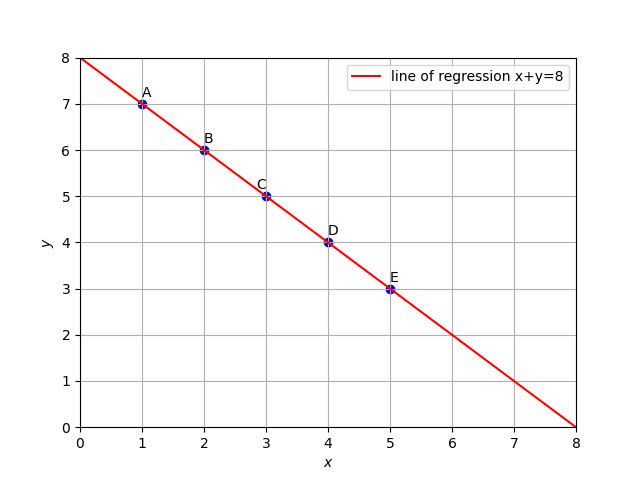
\includegraphics[width=\columnwidth]{./figs/fig1.png}
		\caption{plot of all points}
		\label{Fig1}
	\end{figure}
	
\end{document}